\RequirePackage[l2tabu, orthodox]{nag}
\documentclass{article}

\usepackage[letterpaper, margin=1.3cm]{geometry}
\usepackage{siunitx}
\usepackage{multicol}
\usepackage{mathtools}
\usepackage{amssymb}
\usepackage{mathrsfs}
\usepackage{graphicx}
\usepackage{float}
\usepackage[outputdir=obj]{minted}
\usepackage{pdflscape}
\usepackage{caption}
\usepackage{subcaption}
\usepackage{epstopdf}
\usepackage{filecontents}

\epstopdfsetup{outdir=./obj/}
\usemintedstyle{emacs}
\setminted{linenos,breaklines}
\begin{document}

\begin{titlepage}
	\begin{center}
		\vspace*{1cm}

		\huge{\textbf{Lab 4}}

		\vspace{0.5cm}

		\LARGE{Spectrum Estimation\\of Multimedia Signals}
		\vspace{5cm}

		\Large{\textbf{Michael Kwok (1548454)}}

		\vfill
		ECE 340 Discrete Time Signals and Systems\\
		Department of Electrical and Computer Engineering\\
		University of Alberta\\
		11 November 2020
	\end{center}
\end{titlepage}
\section{Audio Analysis}
\begin{itemize}
	\item Audio Sample Rate: \SI{44.1}{\kilo\hertz}
	\item Audio duration: \SI{22.0297}{\second}
	\item Bits per Sample: 16 bits per second
	\item Bitrate: Bits per Sample \times{} Samples per Second \times{} Number of Channels = 1411200 bits per second
\end{itemize}


\(X[r]\) values:
\begin{itemize}
	\item \(X[0] = -70.04 \) is the DC term, the average of all the samples.
	\item \(X[1] = -41.18 - 28.76j \) is the coeffecient for the \( 0.045 \si{\hertz} \) signal.
	\item \(X[1] = 64.91 + 20.07j \) is the coeffecient for the \( 0.091 \si{\hertz} \) signal.
\end{itemize}

\begin{figure}
	\centering
	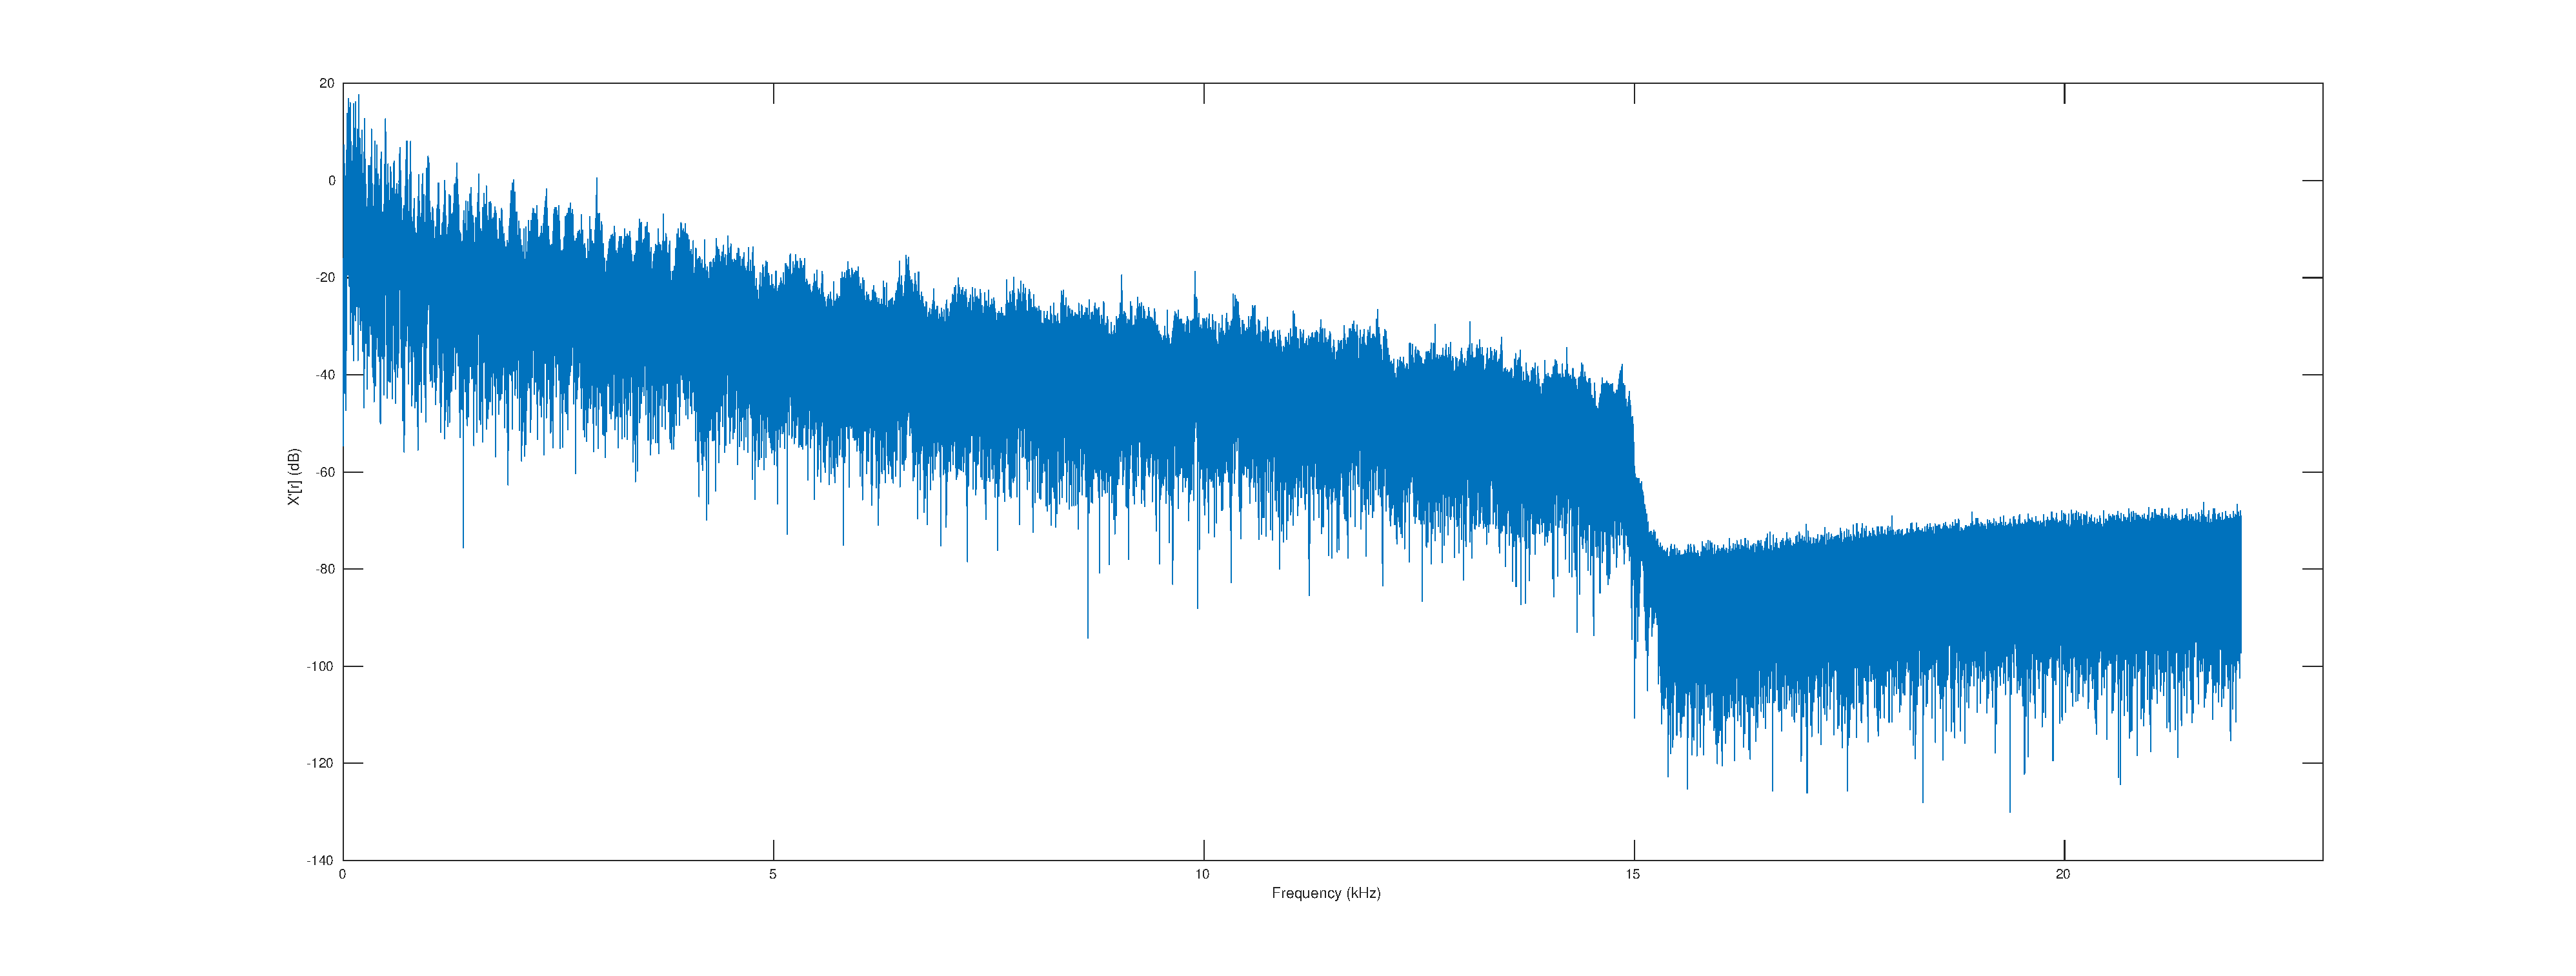
\includegraphics[width=\linewidth]{ubw}
	\caption{Magnitude Spectrum plot of the DFT of ubw}
	\label{fig:ubw}

\end{figure}


The resultant DFT result as shown in Figure~ \ref{fig:ubw} is very noisy, with a big dip in \SI{15}{\kilo\hertz}. The last entry is in \SI{22.05}{\kilo\hertz} which fits the Nyquist Sampling Theorem as the sampling rate is \SI{44.1}{\kilo\hertz}.

\section{Spectrum Estimation}

The frequency range with the most energy is in the range \SI{0}{\hertz} up to \SI{2}{\kilo\hertz}, after which the graph looks like it flattens out with a low energy level.

There's a peak at around \SI{3}{\kilo\hertz}, which is the frequency of the constant beep in the audio file.

\begin{figure}[H]
	\centering
	\begin{subfigure}[b]{0.45\textwidth}
		\centering
		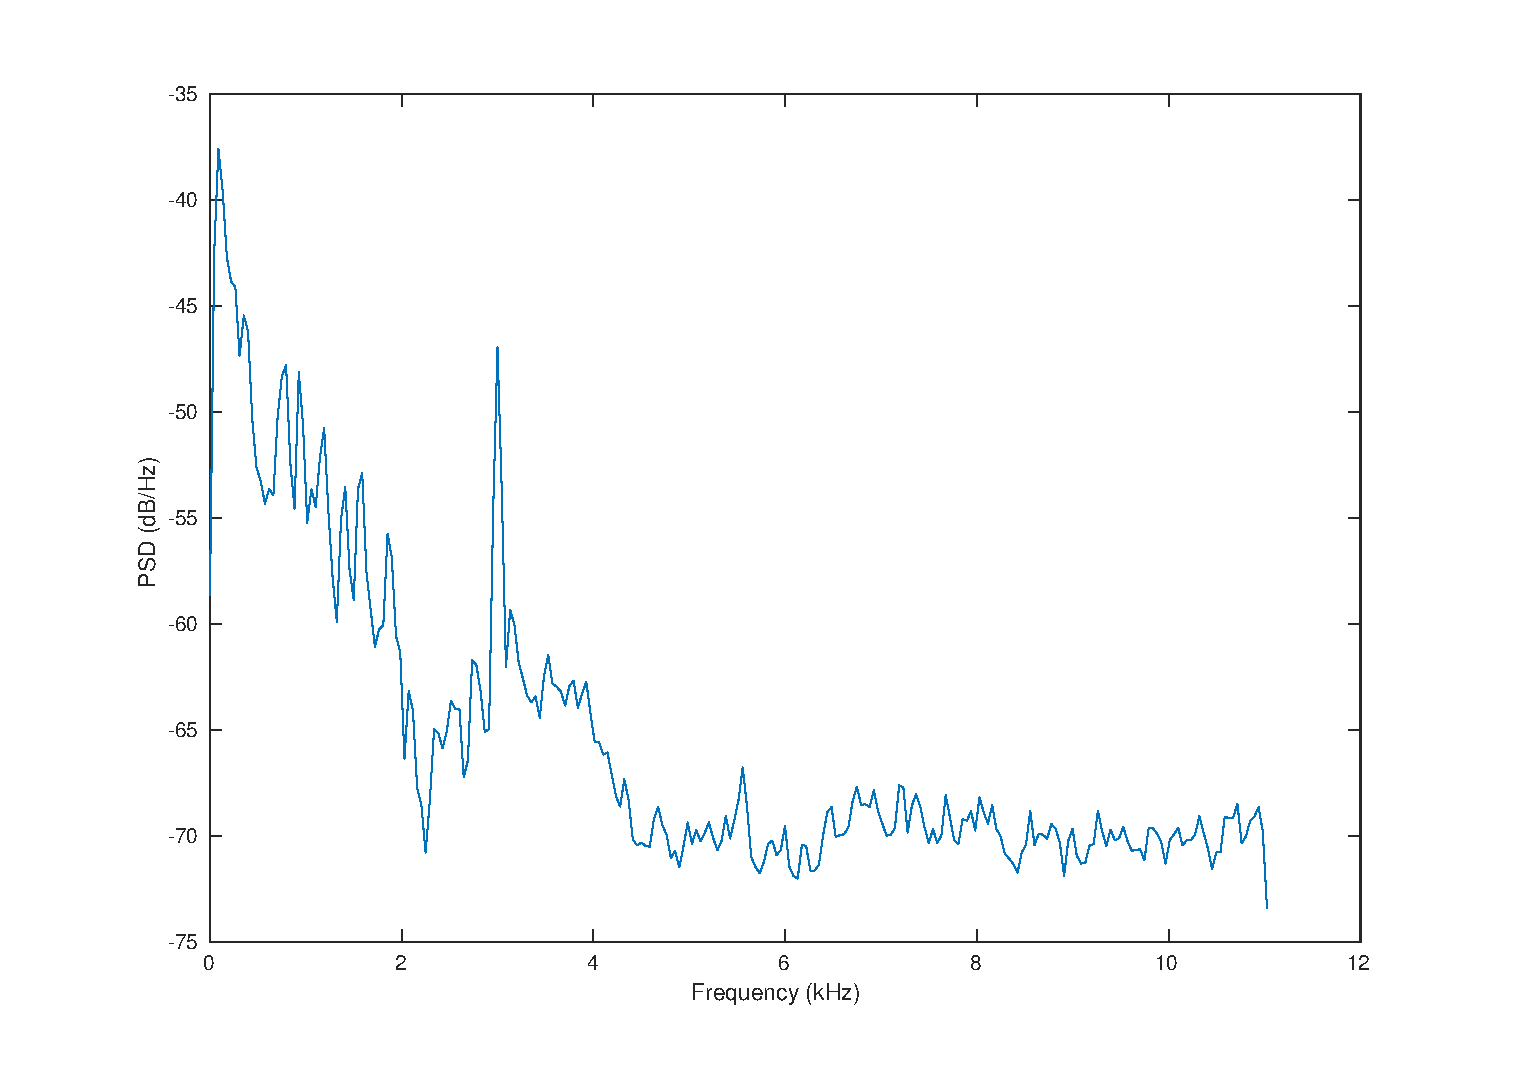
\includegraphics[width=\textwidth]{psd1}
		\caption{PSD plot of lovemono}
		\label{fig:psd1}
	\end{subfigure}
	\hfill
	\begin{subfigure}[b]{0.45\textwidth}
		\centering
		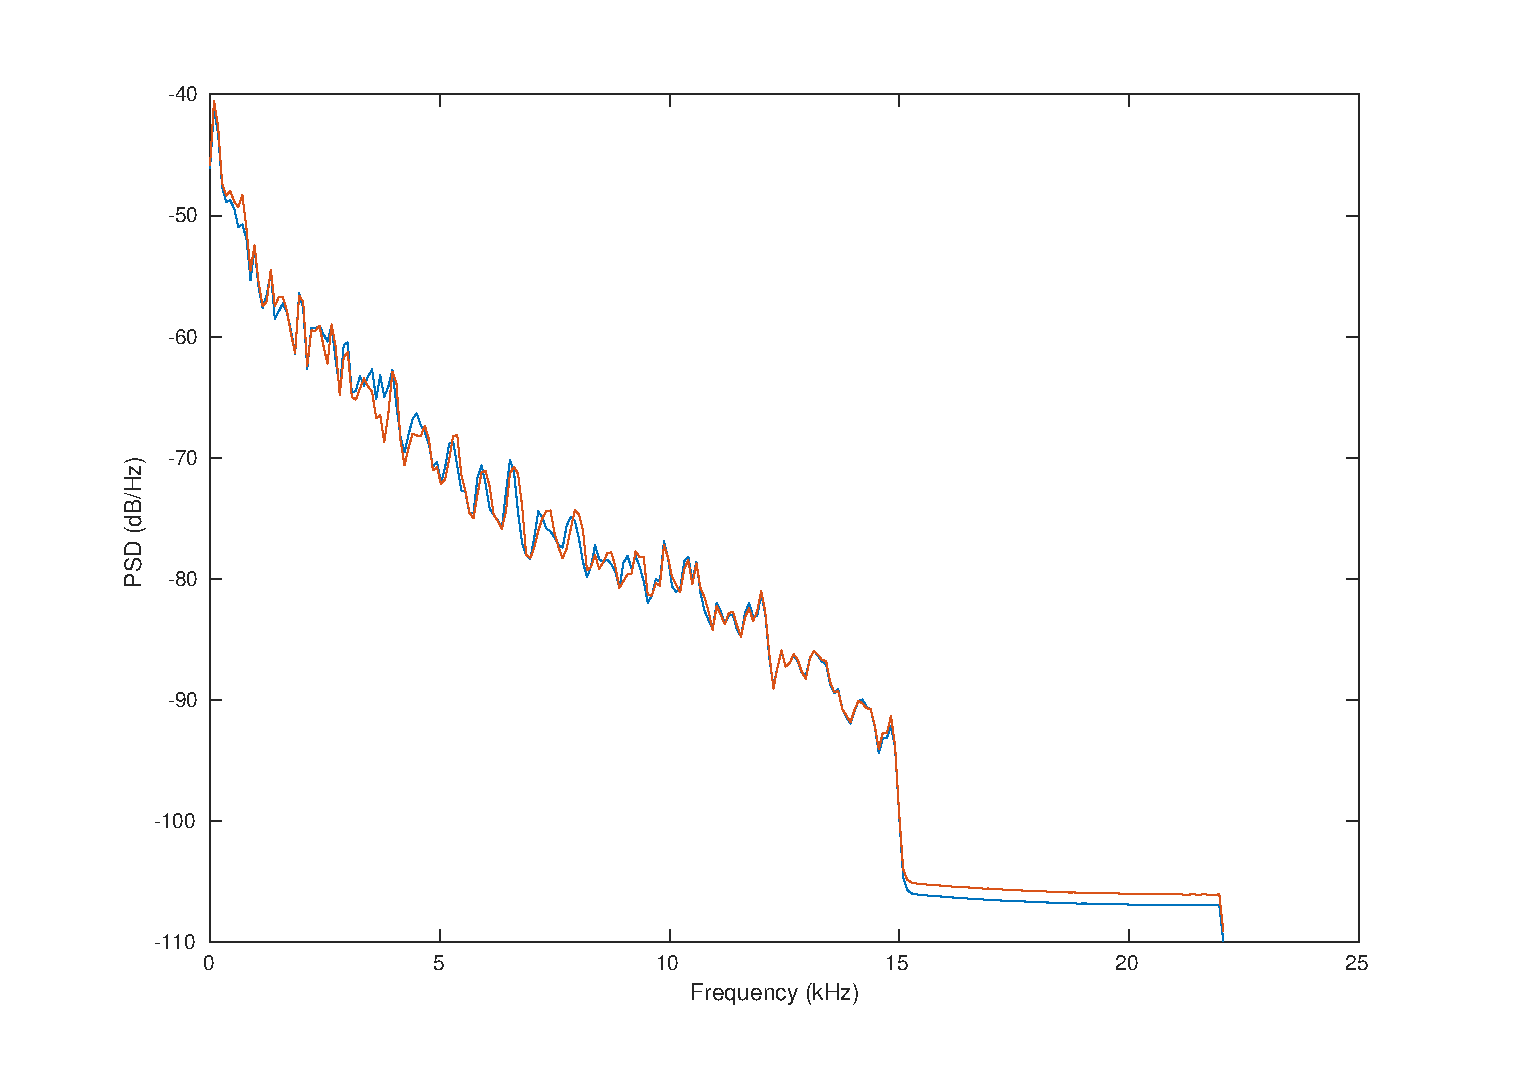
\includegraphics[width=\textwidth]{psd2}
		\caption{PSD plot of ubw}
		\label{fig:psd2}
	\end{subfigure}
	\caption{PSD plots}
\end{figure}

There are two graphs in the PSD plot of \verb|ubw.wav| because that file has 2 channels, left and right while \verb|love_mono22.wav| only has 1 channel.

\section{Image Power Spectrum Diagram}

The image looks like it was subdivided into small squares, as if looking at it through a screen door.

\begin{figure}[H]
	\centering
	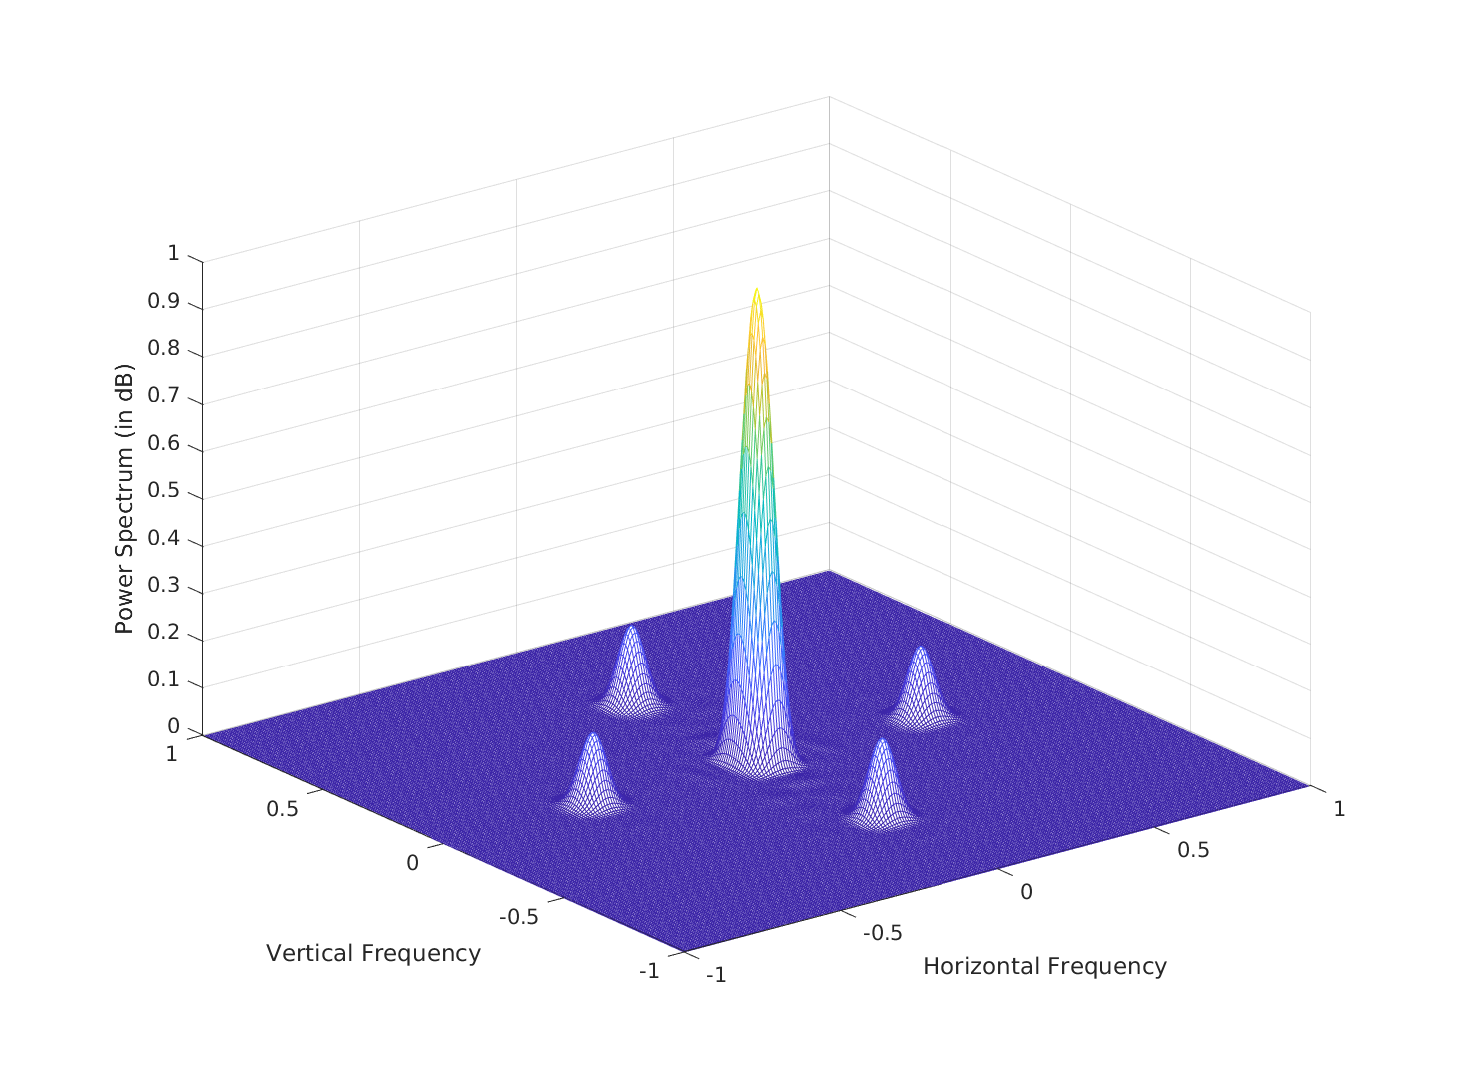
\includegraphics[width=0.5\textwidth]{ipsd}
	\caption{PSD plot of ayantika.tiff}
	\label{fig:psd2}
\end{figure}

The normalized range of both frequencies are between -1 and 1. The noise peaks are at horizontal and vertical frequencies of roughly \(\pm 0.5\).

\pagebreak
\appendix
\section{Complete Code}
\inputminted{Matlab}{Lab4.m}

\pagebreak
\section{Question 4 Code}
\inputminted{Matlab}{Q4.m}

\end{document}
